\chapter{Experimental Methods}
\label{Chap:Methods}

The following Chapter introduces a selection of experimental methods and techniques relevant in the context of the experimental results presented in this thesis and other laser wakefield acceleration (LWFA) experiments. The three main ingredients of an LWFA experiment will be covered: a high-intensity laser, gas targetry and diagnostics for particles and secondary radiation. The measurement of high-energy gamma radiation will be discussed more extensively as it is central to this work.

The Chapter starts by introducing the \textsc{Gemini} laser system, the dual-beam high-intensity laser used to conduct the experiments in this work, along with diagnostics and methods used to characterise high-intensity laser pulses.
It then continues with a section on gas targets used in this work and techniques to diagnose the plasma, followed by particle diagnostics.
Finally, the chapter focuses on diagnostics for high-energy radiation in the gamma regime, in particular a scintillator array used to infer gamma spectra.
A comprehensive review of diagnostics used in LWFA experiments is, for instance, provided in \cite{Downer2018_DiagnosticReview}.

\section{The Gemini laser system}

All of the experimental results presented in this work were acquired at Target Area 3 using the \textsc{Gemini} laser \cite{Hooker2006_Gemini,Hooker2008_Gemini} of the Central Laser Facility at the Rutherford-Appleton Laboratory, UK.

\subsection{Laser properties}

The titanium-sapphire \textsc{Gemini} laser system with central wavelength $800\,\mathrm{nm}$ provides two beams every 20 seconds at a compressed pulse duration of down to $30\,\mathrm{fs}$ and up to $15\,\mathrm{J}$ energy on each arm \cite{GeminiWebsite}. The collimated beams that enter the target chamber have a diameter of just under $\sim 150\,\mathrm{mm}$ with a flat-top intensity profile and are focused with a spherical mirror or off-axis parabolas (OAPs). Adaptive optics (AOs) are deployed on both laser arms in conjunction with wavefront sensors to remove aberrations and flatten the wavefront.
In addition to its full-power capabilities, a continuous-wave mode for alignment and a low power pulsed mode at 10 Hz repetition rate are available.

%\EliasComm{Vacuum compressors, gate valves. CPA. Separate laser and target area.}

%\subsection{Target Area 3}

%At \textsc{Gemini} the laser and the target area, called Target Area 3, are located in the same building but separate rooms.
%The target area 
%\EliasComm{Rough dimensions. Dimensions of vacuum chamber. Extension chambers. Lasers around the centre. Motivate dimensions. Bunker dimensions are $8 \times 8$ m and 1 m thick walls and 0.6 m concrete roof, along with lead shielding.}

\subsection{Beam line geometries}


\begin{figure}
\centering
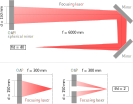
\includegraphics[width=0.8\columnwidth]{BeamGeometries.pdf}
\caption{Sketch of relevant focusing geometries used in experiments at \textsc{Gemini} discussed in this work. Top: A long-focal-length geometry using an $f/40$ spherical mirror or off-axis parabola used to drive a wakefield accelerator. Bottom: A short-focal-length $f/2$ geometry for a scatterer or heater beam using a full off-axis parabola (left) or an optic with a central hole (right).}
\label{Methods:Figs:FocusingGeometries}
\end{figure}
In the context of the LWFA experiments discussed later typically two types of beam line geometries are of relevance at \textsc{Gemini} (see Figure \ref{Methods:Figs:FocusingGeometries}):
First, a long-focal-length geometry using either an $f/40$ spherical mirror or an off-axis parabola with $f = 6\,\mathrm{m}$ to provide an intense laser pulse $a_0 > 1$ with a long Rayleigh length, $z_R$, to efficiently drive LWFA over long distances. This geometry is used in all experiments discussed in this work. Due to the long focal length and the limited size of the target area and the vacuum chamber the beam has to be reflected or `folded' at least once during the focusing process, in recent setups about halfway between optic and focal plane. As a result, the maximum usable energy in this laser arm is limited by the damage threshold of these `folding' mirrors or in other words the fluence (optical energy delivered per unit area) the mirrors can sustain. The threshold at which damage occurs depends on several factors, including the beam quality and beam size, the quality of the mirror coating and cleanliness of the chamber.

The second focusing geometry is the short-focal-length scatterer which is typically an $f/2$ off-axis parabola with focal length $f = 300\,\mathrm{mm}$. In the experiments discussed in Chapters \ref{Chap:linICS} and \ref{Chap:RR15} an off-axis parabola with a central fitted hole was used to enable a head-on counter-propagating geometry in conjunction with the long-focal-length beam line. 


\section{Laser Diagnostics}


\subsection{Laser Energy}

At \textsc{Gemini}, the laser energies are measured on every shot by collecting the transmitted light through the back of a highly-reflective dielectric mirror in the laser area and imaging it onto a CCD camera chip. The integrated number of counts on the CCD is calibrated using a laser energy meter (Gentec QE8SP-B-BL-D0) and the filtering is adjusted for different power modes.
A laser energy meter is also used to measure the reflectivity of the compressor gratings, at \textsc{Gemini} typically between 60 and 70 percent, and the energy reaching the interaction point.

\subsection{Laser Pulse Duration}

At \textsc{Gemini}, frequency-resolved optical gating (FROG) \cite{FROG} is used to measure the pulse duration of the laser and characterise its temporal intensity profile.
A FROG trace is taken on every shot by collecting laser light that is transmitted through highly-reflective dielectric mirrors.

The FROG is a diagnostic to measure the intensity and spectral phase of ultrashort laser pulses as present at \textsc{Gemini} ($\sim 40\,\mathrm{fs}$). The setup is similar to an autocorrelator and is optically gated by combining two beams in a non-linear medium, typically a second-harmonic-generation crystal. The radiation is then spectrally resolved (hence frequency-resolved) and provides information about the spectral phase. See, for instance, \cite{FROG} and \cite{StreeterThesis} for more details.

\subsection{Focal Spot Characterisation}

\EliasComm{Replace this with 3 focal spot images (f/40, f/2 and f/2 with phase plate) on intensity scale. Then in words describe how to get there: take image on low power modus, then assume that it remains the same in shape. Measure energy and pulse duration, peak power on-shot and use that to derive an intensity map. Also give an estimate how close the low-power focal spot and the high-power focal spot is. The first three amplification stages are the same. On-shot final stage is mistimed.}
In LWFA a short-pulse laser is focused down to reach high enough intensities to drive a wake, but has to guide itself over a long range at the same time. In parts of this work a second laser is used as scatterer for inverse Compton scattering or as an X-ray heater.

For each of these applications it is important to optimise and characterise the size and spatial energy distribution of the focal spot. Combining this with a measurement of the temporal pulse shape, for instance using a FROG, then provides an intensity map of the laser pulse at focus.
\vspace{\baselineskip}

In this work a CCD camera (AVT Manta G-033B) is coupled to a near infrared infinity-corrected apochromatic long-working-distance microscope objective (depending on the application Mitotoyo $\times10$ or $\times20$ magnification) to image the spot at its focal plane. 
A thin metal wire of $10's-100 \,\mathrm{\mu m}$ width is used to help define a focal plane.
\vspace{\baselineskip}

Due to the high intensity \textsc{Gemini} can reach the beam alignment is performed in the CW mode and the focal spot is characterised with an attenuated low-power pulsed beam. Assuming the focal plane and general character of the spot remains the same in the attenuated beam, the energy of the actual focal spot on shot is then scaled from the low power image.
\SMComm{Make sure you distinguish between CW alignment and pulsed/high power focal spot. CW and high power spots are not the same.}

A real direct measurement of the actual focus at typical intensities used in wakefield experiments is very challenging. Recent attempts involved the full 3D characterisation of the wavefront of the collimated laser beam by applying an asymmetric Mach-Zehnder interferometer and scanning the entire beam profile over hundreds of shots \cite{TERMITES} or using a gas jet ionisation (REF HERE)\addref. 

\begin{equation}
a_0 \approx 0.85 \lambda [\mu m] \sqrt{I [10^{18} cm^{-2}]}
\end{equation}

\SMComm{I think you need to say a little more about how close the focal spot is. The key thing is that the first three amplifications....}
\subsubsection{Image Processing}

In addition to a spatial calibration, the images for a focal spot analysis require some background removal: 
A series of images without any laser are taken (dark field) and averaged over to be then subtracted from the actual focal spot image. 
Then a median filter can be used to account for individual hot pixels on the camera.
\SMComm{Too much detail?}
The remaining signal should be mainly the laser spot and the highest pixel values are at the centre of the focal spot.
Taking the maximum pixel value and fitting an ellipse to area reaching half of this value, the \textsc{fwhm} size of the spot is estimated.
The area of the focal spot, ignoring smaller deviations from an ellipse, is then $A = \pi a b$, where $a$ and $b$ are the two axes.
Comparing the pixel counts within the \textsc{fwhm} contour against the pixel counts in the total beam, one can then quantify the fraction of energy contained in the \textsc{fwhm} the beam. A high fraction is important as the wings of the beam decreases the peak intensity and will not be guided in the wakefield accelerator, is hence lost.
\SMComm{Reference? Mangles PRSTAB and Genoud...}

\subsubsection{Spatial calibration}

As the exact size of the focal spot is important, the focal spot camera has to be spatially calibrated. Carefully measuring the distances between the components of the optical system and knowing about their properties might not be accurate enough. Alternatively, the camera can image an object of well-defined spatial extent. A typical tool are USAF targets, for instance provided by Thorlabs, available in transmissive or negative, with a range of line sets of different dimensions. Knowing the pixel size of the camera one can then relate the width of the lines to a conversion factor from pixels to microns, in this case. Another approach is placing a grid of known dimensions into the collimated laser beam and deduce the spatial dimensions by measuring the separation of the diffracting multiple copies of the focal spot following:
\begin{equation}
\sin \theta = \frac{m \lambda}{d} \rightarrow x_m = m f \tan \theta \rightarrow x \approx \frac{f \lambda}{d}
\end{equation}

\SMComm{References for these things?}

\subsubsection{Intensity Estimate}

Knowing about the total energy in the beam and combining this with a measurement of the pulse shape (e.g. using a FROG), the number of pixel counts in the spot can be related to an intensity in the beam.
The focal spot in figure XXX for instance has a size of XXXXXXX. The FROG analysis indicates a peak power of XXX TW. Combined this gives a peak $a_0 = 2$. 
\SMComm{Errors, for which experiment, OAP...}
Ideally, a series of several focal spots, even hundreds, are taken to incorporate fluctuations in the shape of the spot but also to characterise the typical spatial fluctuations over time.
\SMComm{Add figures of laser intensity for a0, f/40 f/2 and with phase plate?}


\section{Dual-Beam Timing Diagnostics}
\label{Methods:Sec:DualBeamTiming}

\SMComm{I think this section needs more background information for the reader who isn’t familiar with what you are trying to do.  
 we need to time two beams to femtosecond level which cant be achieved with diodes.
interference can be used (time scale of the pulse envelope)
well known inteference patterns  for two plane waves crossing at an angle (straight fringes) or plane wave and spherical wave front (circular fringes) 
 also get similar for large f number and small f number expanding beams which is suited here.}
 
In experiments involving two or more pulsed laser beams, for instance pump-probe or colliding-pulse experiments, the beams require spatial and temporal synchronisation down to the picosecond or even femtosecond level.
Depending on the accuracy required different techniques can help measure the difference in timing, as well as correct and monitor the synchronisation over extended periods of time.

Photodiodes, spatial and spectral interferometry are introduced. This is not an exhaustive list and other methods, e.g. cross-correlator, are not introduced as they were not used explicitly in the experiments presented.
\vspace{\baselineskip}

At \textsc{Gemini} both laser beams originate from the same source (oscillator) and are hence `intrinsically' synchronised, which means that they are emitted/triggered at the same time, underlie the same jitter but do not shift relative to each other at the point of emission (SM: GRAMMAR). However, this does not mean that both beams are automatically synchronised at the point of interaction, since the arms take different pathways through the amplification and compression stage, and then finally follow different beam lines within the target chamber. The longer their separate paths the larger the potential impact of, for instance, vibrations and thermal effects can be. Small changes can cumulatively make a significant impact on the femtosecond-scale synchronisation required in some of the challenging experiments attempted at \textsc{Gemini}.
\vspace{\baselineskip}

`Timing' two beams means in this case that the relative path lengths are adjusted to compensate for the measured difference in the time of arrival at the interaction point. At \textsc{Gemini} larger distances (few nanoseconds or metres in distance) require moving optics physically to extend the beam path, smaller distances are finely adjusted by using a linear translation stage that adds or removes path length in double-pass at few femtosecond (micrometre) precision. This stage is on the `split-and-delay' table in the LA3 laser area. The linear stage is a Newport XXX REFat XX precision\addnum\addref.

\subsection{Photodiodes}

Photodiodes are a useful and easy-to-use tool to measure the temporal separation of light signals on a nano- to picosecond scale.
Rise and fall times for fast diodes are few tens of picoseconds placing the peak of the distribution within $\sim10\,\mathrm{ps}$ using an appropriate oscilloscope. 

Both laser pulses have to be overlapped at the designated point in space and the signals combined onto the diode. Alternatively, an object at the crossing point can be used to scatter both beams to send a more diffuse signal to the diode. This is a suitable method if the extent of the scattering object is negligible on the order of the accuracy of the method.
\vspace{\baselineskip}

\begin{figure}
\centering
\includegraphics[width=0.3\columnwidth]{PhotoDiode_BW.jpg}
\caption{Photodiode.}
\end{figure}

In the experiments at the \textsc{Gemini} laser the fast EOT-4000 GaAs photodetector with a rise/fall time of $< 30\,\mathrm{ps}$\footnote{Details can be found on the Electro-Optics website. www.eotech.com} was used in conjunction with a Lecroy WaveMaster 813Zi-B oscilloscope ($>13\,\mathrm{GHz}$)\footnote{More details on Lecroy XX WEBSITE XX}. This limits the resolution of the signal to about XXX PS. The accuracy of the difference measurement is per measurement is a few picoseconds. If several measurements at different separations (using a delay stage to delay one laser arm) are taken the error can be reduced to an accuracy of XXX PS\addnum{}.
The detectors were only used at air and are not compatible for vacuum use.
\EliasComm{This is also as we need short and thin cables to make use of the fast oscilloscope and this would not work with a feedthrough. Why is this}
\EliasComm{Add details here (see results chapter)}
\EliasComm{Replace footnotes by references or similar as they look like squares etc.}
\EliasComm{Add data (we have the excel sheets for this).}
\EliasComm{Do we have proper data from the scope.}

\subsection{Spatial Interferometry}
\label{Methods:Sec:SpatialInterferometry}

Diode timing is limited by the typical rise and fall times and the access to a fast oscilloscope.
A different method that is more coupled to the pulse duration of the laser beams is spatial interferometry. 
If both laser pulses have the same polarisation and are overlapped in space and time, they can interfere. 
Due to the large bandwidth of the Ti:Sa laser pulses used in this context the coherence length is very short and interference will only take place over the combined pulse duration, i.e. a potentially small time window. This is why this method is a useful technique to achieve precise timing after using a diagnostic with a wider time window (but less precision) like the photodiodes introduced in the previous section.

\SMComm{This sentence comes across as a bit confused.   Is it the pulse duration or the bandwidth that determines the coherence length? }
\begin{figure}
\centering
\includegraphics[height=0.4\columnwidth]{Fringes_spatial_F2F20.png}\includegraphics[trim={14cm 0 0 0}, clip,height=0.4\columnwidth]{Fringes_spatial_exp.png}
\caption{Fringe simulation and experimental results for f/40 and f/2.}
\end{figure}


\EliasComm{Add here an example for Gaussian beams and the equation for interference based on this. Proper explanation}

\begin{equation}
\boxed{I \sim |1+\cos(ky \sin\theta - \omega \Delta \tau + \phi )|}
\end{equation}
\SMComm{Relate to the equation.}

As we see the interference fringes rely on a phase difference between the two laser pulses. The main contributor for two timed spectrally identical laser pulses are a relative angle or different radii of curvature.
The experiments presented combine a short focal length optics with a longer focal length beam line and hence perfect alignment can be aspired to as the interference pattern will be clearly visible due to the stark difference of the radii of curvature of, for instance, and f/40 and f/2 at the relevant point.
\EliasComm{Change perfect alignment for something else.}
\SMComm{Replace figure by sketch and adjust the fringes so that the simulations match orientation?}

\subsubsection{Experimental Implementation}

In the experiments described in Chapters RR15 XX and RR19linICS XX spatial interferometry was used. 
Both beams were reaching the interaction point at 180 degrees from each other. One f/2, the other f/40. A 90-degree knife-edge prism with reflective surface was driven in at the desired interaction point and used to deflect both beams collinearly onto the CCD chip of a camera, in this case equipped with a x10 long-working-distance microscope objective.

The contrast of the interference pattern was adjusted by equalising the relative brightness of the beams with a combination of adjusting the distance of the camera to the prism edge taking advantage of the different focal lengths and by adjusting the rotation angle of the polariser as the beams are cross-polarised.
These measurements were done using the pulsed low power beam at \textsc{Gemini}.
\SMComm{Results?
Can you show plot of fringe visibility v delay? 
How accurately can you time beams?}

\subsection{Considerations for Synchronising Beams}

Synchronising two laser beams to each other or a laser with an electron beam in an experiment down to the femtosecond level comes with many challenges and considerations.

Light moves slower through media than through vacuum. The group velocity, $v_g$, is reduced by the refractive index, $\eta$, to $v_g =c/\eta$ or more specifically in a plasma to $v_g \approx c(1-1/2 (\omega_p/\omega)^2)$ (see Section \ref{Theory:Sec:LaserPropagationPlasma}), where $\omega$ is the frequency of the laser and $\omega_p$ is the plasma frequency (see Section \ref{Chap:Theory:Sec:PlasmaFreq}).
Introducing or removing media asymmetrically from beam paths changes the relative time of arrival of laser pulses.
Typical examples at \textsc{Gemini} for this are moving from air to vacuum (pumping down the vacuum chamber), opening or closing the transparent gate valves, or attenuating beams using glass slides when switching between different power modes.

\subsubsection{Shifting beam paths from air to vacuum}

The refractive index of vacuum is $\eta_0 = 1$, whereas the refractive index of air, for instance, at $20^\circ$ Celsius, $45\%$ relative humidity and atmospheric pressure for light of wavelength $\lambda = 800\,\mathrm{nm}$ is $\eta_{air} = 1.00027$ \cite{Stone2011_ETAAIR}. The difference in time, $\Delta t$, it takes a laser pulse to travel a distance $d$ in vacuum or air is then proportional to the difference in the refractive indices:
\begin{align}
\Delta t &= \frac{d}{c} \left( \eta_{air} - \eta_{0}\right),\nonumber\\
\Delta t  &\approx 0.9\,\mathrm{ps} \times \frac{d}{1\,\mathrm{m}},
\end{align}
which means that it takes the laser pulse $0.9\,\mathrm{ps}$ longer to travel one metre in air than in vacuum.
If the beam paths of two laser pulses are of different length, the difference in their beam path will result in a shift in the relative time of arrival at the interaction point when transitioning from air to vacuum.

At \textsc{Gemini} the laser arm used as wakefield driver typically covers a beam path of over $10\,\mathrm{m}$ distance due to the long-focal-length geometry with $f = 6\,\mathrm{m}$, whilst the scatterer beam only covers about half of the distance. If both beams arrive at the same time at the interaction point when the chamber is at air, then a difference in $5\,\mathrm{m}$, for instance, would mean that in vacuum the laser pulse following the long-focal-length beam line arrives at the interaction point $4.5\,\mathrm{ps}$ after the scatterer.
\vspace{\baselineskip}

As a result of the pump-down process the components in the vacuum chamber and the vacuum chamber itself experience changes in pressure and temperature which in turn result in stress on the materials. This can lead to a steering of the laser beams which affects the alignment in general but also modifies the beam path.

\subsubsection{Opening and closing gate valves}

Another step in the pump-down process at \textsc{Gemini} is opening the gate valves that separate the target chamber, which is often at air or lower quality vacuum, from the relatively permanent and high quality vacuum of the two laser compressors.
Once the pressure in the target chamber reaches a sufficiently low value and the turbo pumps are engaged, the gate valves can be opened.
Both gate valves at \textsc{Gemini} are made of sapphire glass, but measurements found a slight difference in thickness of around $\Delta x = 60 \pm 3\,\mathrm{\upmu m}$ \cite{GEMINI_GATEVALVES} corresponding to $\Delta t = 350\pm17\,\mathrm{fs}$ at a wavelength of $\lambda = 800\nm$. The gate valve of the laser arm that is predominantly used as wakefield driver was found to be thicker.

\subsubsection{Attenuation of beams}

The previous two examples can be cross-checked by repeating some of the timing procedures after the pump-down, for instance using again spatial interferometry.
At \textsc{Gemini} glass slides are used as beam attenuators in the low-power modes and can be used in conjunction with polarisers and waveplates to improve the contrast of the interference pattern in spatial interferometry (see Section \ref{Methods:Sec:SpatialInterferometry}). In some cases this will require inserting material asymmetrically in both laser arms in order to optimise the visibility of the pattern.

The attenuators are $2\,\mathrm{mm}$ thick fused silica glass slides with refractive index $\eta = 1.4533$ \cite{Malitson1965_FusedSilica}. The slides are inserted at 45 degrees angle relative to the laser beam axis which delays the laser pulse by $4.24\,\mathrm{ps}$ for each glass slide. The attenuators were found to be identical to each other to within $\Delta x < 10\microns$, such that an equal number of attenuators in each beam path does not introduce a relative delay. An unequal number of attenuators in each beam, on the other hand, requires an adjustment of the beam paths after `synchronising' the beams using spatial interferometry.

\subsubsection{Synchronisation of an LWFA electron beam with a laser pulse}

So far the considerations and methods have been aimed at ensuring the temporal overlap of two laser pulses, taking into account changes introduced by pump-down procedures or attenuation. Finally, we want to highlight what to consider when aiming to synchronise a laser pulse to an electron bunch accelerated through LWFA, relative to a laser-laser synchronisation.
\vspace{\baselineskip}

In LWFA, the driver beam propagates through a plasma and is hence slower relative to the in vacuum-timing procedure: it will arrive later at the interaction point than measured previously in vacuum.

The electrons are injected after a certain distance of propagation. At injection they quickly reach a velocity close to the speed of light, from when the electrons and the second laser pulse travel at approximately the same velocity.

For the relative offset of the driver pulse and the electron bunch we can estimate that the bunch trails in the Nth bubble behind the laser pulse between N/2 to N plasma wavelengths, the accelerating to zero phase region of the bubble. If the electrons are close to dephasing and in the first bubble, the laser-electron offset is 1/2 $\lambda_p$.
\vspace{\baselineskip}

This shows that knowing the point of injection becomes important. Alternatively, calculate the distance the laser pulse propagated in plasma and take this as total delay (as the electrons are moving just as fast as the laser in vacuum from thereon forwards). For this purpose measuring injection radiation or forcing radiation at a designated point (shock injection) becomes very useful.

However, this assumes that the electron bunch does not have a spatio-temporal extent which is typical for LWFA beams with long tails and potentially energy-time chirp. Short, localised injections will lead to low energy spread but also short bunches that will localise the beam further. This is also a property shock injection can facilitate.
\EliasComm{Rephrase.}
\SMComm{Maybe put a typical number in this - at density x this corresponds to a delay if y fs }
\SMComm{I was trying to decide if this was better in methods or the RR chapter.  Either will work, and I like it here,  but the effect needs to be mentioned in the results too}
\SMComm{Numbers?  You say knowing the injection point is important,  can you quantify?  Extreme worse case would be injection anywhere in the accelerator. But it will be significantly better than this!}

\subsubsection{Stability of synchronisation over extended periods of time}

\begin{figure}
\centering
\includegraphics[width=0.8\columnwidth]{Shalloo_TimingDrift.pdf}
\caption{Change in delay between the two laser arms measured in the target area using a spectral interferometry setup as a function of time (moving average in red line). The relative changes in temperature as measured in the laser area are shown in blue. Reprinted from \cite{Shalloo_GEMINIDRIFT} with permission of the author, R. Shalloo.}
\label{Methods:Figs:ShallooTiming}
\end{figure}

After having discussed some of the considerations related to achieving a temporal synchronisation of two laser pulses, or a laser pulse and an electron beam, we will now consider the challenges associated to maintaining this synchronisation over an extended period of time.
At \textsc{Gemini}, the laser pulses propagate typically several 10's of metres distance across mutiple laser areas before being directed into the target area. Minor changes in the environment, e.g. humidity or temperature, can lead to an expansion or contraction, for instance, of optical tables and optics mounts leading to a drift of the alignment and the relative timing over a period of time. In Figure \ref{Methods:Figs:ShallooTiming} the relative delay between the two \textsc{Gemini} laser beams in the target area is shown as a function of time (red) along with variations in the temperature in the laser area (blue) \cite{Shalloo_GEMINIDRIFT}. The measurements indicate fluctuations in the relative delay of $> 100\fs$ over the course of $\sim 20$ minutes associated with temperature changes of $\sim 1^\circ$ Celsius. This highlights the importance of a stable environment in the laser and target area to ensure that the sensitive alignment and synchronisation can be maintained for longer periods of time, but also indicates that it is crucial to monitor and identify drifts as seen in Figure \ref{Methods:Figs:ShallooTiming}.


\section{Gas Targets}

In laser-wakefield acceleration (LWFA) the laser pulse propagates through a plasma and sets up a density modulation. This requires a plasma with a density below the critical density, $n_c = m_e \epsilon_0 \omega^2/e^2$. A medium with electron density $n_e < n_c$ is referred to as `underdense'. For a laser of wavelength $\lambda = 800\,\mathrm{nm}$ these are typically gaseous targets. `Overdense' targets with a density higher $n_e \geq n_c$ are for titanium-sapphire lasers mostly solid or liquid targets used for ion acceleration schemes, e.g. (Target Normal) Sheath Acceleration \cite{Wilks2001_IONACC,Maksimchuk2000_IONACC}, or to generate X-rays \cite{Edwards1990_BURNTHROUGH}. 
\vspace{\baselineskip}

Gas and liquid targets can be destroyed and replenished in a short amount of time without significant re-alignment and debris production, and are suitable for high-repetition experiments. The factors limiting the repetition rate are then the performance of the vacuum system, the time it takes the gas flow or liquid to reach equilibrium, the durability of nozzles and other components, and the repetition rate of the laser system itself.
\vspace{\baselineskip}

Examples of gas targets that are routinely used for wakefield experiments are gas jets \cite{Semushin2001_GASJETS}, gas cells (REF\addref) and capillaries \cite{Spence2001_WAVEGUIDE,Leemans2006_GEV}. In some cases several targets of the same or different type or combined and staged together to achieve more favourable results (REF\addref). The target size, i.e. the distance the laser pulse propagates through the medium, has to be matched with the laser in use, considering depletion and dephasing lengths to optimise the particle and radiation output, and to use the energy of the laser pulse efficiently. As a result, there is a large variety of different targets, each tailored to a different application (REF\addref). Here we will focus on examples of gas jets and cells relevant to the work presented within the course of this thesis. An overview of those targets is given in Table \ref{Methods:tables:GasTargets}.

\begin{figure}
\centering
\includegraphics[height=0.35\columnwidth]{GasCell_Example_cut.png}\includegraphics[height=0.35\columnwidth]{conical_nozzle_prettypic.jpg}
\caption{Gas targets under fire. Right: Picture of a diverging supersonic gas jet with $15\,\mathrm{mm}$ diameter. The emerging helium gas is ionized by the laser and lights up. Picture taken at \textsc{Gemini}, Central Laser Facility, in December 2015. Left: Gas Cell}
\end{figure}

\begin{table}
\centering
{\rowcolors{3}{white}{lightgray!50}
\begin{tabular}{|r|r|r|r|r|}
\hline
\multicolumn{5}{|c|}{\textbf{Gas Targets used in this work}} \\
\hline \hline
\textbf{Chapter} & \textbf{Target Type} & \textbf{Length} & \textbf{Gas} & \textbf{Inj. Mechanism}\\ \hline \hline
\ref{Chap:linICS} & Jet + Blade & 15 mm & Helium & Shock Injection\\
\ref{Chap:RR15} & Jet & 15 mm & Helium & Self + Shock Injection\\
\ref{Chap:BW} & Cell & 20 mm & Helium + N & Self + Ionisation Injection\\
\hline
\end{tabular}
}
\caption{Overview of gas targets and gases used in this work.}
\label{Methods:tables:GasTargets}
\end{table}

\subsection{Gas Jets}

The flow of gas produced when forcing it with high backing pressure through a small orifice at the bottom of a diverging cone is in the context of this work related to as gas jet.
\SMComm{awk}
If the measurements of the cone are chosen correctly at a high enough backing pressure, the flow detaches and becomes supersonic \cite{Semushin2001_GASJETS}. 
\SMComm{detaches from where, jargon. Why are short ramps preferable? }
Supersonic gas jets are able to produce relatively smooth flat-top density profiles with short density ramps on both sides, suitable for LWFA.

The density of the gas jet is controlled by varying the backing pressure of the gas line, where higher pressure results in higher densities. When comparing nozzles of the same type in different sizes, larger nozzles require higher backing pressures to reach the same densities as smaller nozzles. For supersonic flat-top profiles the density slowly decreases above the nozzle. The actual density profile and gas flow depends on the specific design and manufacturing.
\vspace{\baselineskip}


Gas jets provide a relatively easy target, diverse in shape and comparatively straightforward to align. The open geometry also allows optical probing from a large solid angle. However, experimental results tend to be less stable (shot-to-shot reproducibility) and inferior in terms of maximum energy \cite{Leemans2014_GEV} and stability \cite{Desforges2014_CAPILLARY,Osterhoff2008_CELL} to setups relying on gas cells or capillaries at similar conditions, especially at low densities, as the medium is laminar and reproducible. ALSO MENTION MAX ENERGY FROM JET (4 GEV CORELS) \cite{Kim2013_GEV} \SMComm{too definitive.  Improvements could also be for other reasons... }
\vspace{\baselineskip}


Different geometries and nozzles are being used depending on the application: for instance conical and rectangular, completely flat or double cones, diverging or converging. Different nozzle types and sizes have advantages for certain applications, producing density profiles for enable specific injection mechanisms, provide a fairly smooth flat-top profile \cite{Semushin2001_GASJETS} and so on.
The diversity of nozzle designs also lead to the idea of using 3D printing methods for fast prototyping and tailoring the nozzles to the specific needs of the experiment \cite{Jolly2012_3DJET}.

To tailor the density profile even more groups have inserted thin objects into the supersonic gas flow to induce a shock front. The shock introduces a sharp density transition in the density profile which can be used to trigger a localised injection event in LWFA referred to as shock injection \cite{Schmid2010_SHOCK,Buck2013_SHOCK}.

The material applied is frequently a type of metal, varying from aluminium to steel or brass, in order to withstand the high laser intensities and the plasma heat. In the case of \cite{Jolly2012_3DJET} plastic was used for prototyping. Manufacture errors or deterioration over long run times can have an impact on the gas flow and will lead to deviations from idealised hydrodynamic simulations. Hence nozzles (and other gas targets as well) are usually characterised, i.e. their gas flow is analysed, either before or after an experiment to account for deviations from the ideal simulation properties in hydrodynamic codes. The density can, for instance, be determined using an interferometry setup and Abel inversion \cite{FOURIER}.



\subsubsection{Experimental Implementation}
\begin{figure}
\centering
\includegraphics[height=0.3\columnwidth]{TopView_Blade_Gas_S_Edge.jpg}\includegraphics[height=0.3\columnwidth]{Blade_interferometry_reference.jpg}\includegraphics[height=0.3\columnwidth]{ShadowgraphyXiao.jpg}
\caption{Gas jet with blade example pics. Shadowgraphy by Xiao Cui (MSc Imperial College).}
\end{figure}
The gas nozzles used in the experiments discussed in Chapter \ref{Chap:linICS} and \ref{Chap:RR15} are conical aluminium nozzles designed to produce supersonic gas flows. The nozzles were operated at 70 to 100 bar backing pressures, providing electron densities of few $10^{18}\,\mathrm{cm}^{-3}$. The orifice size, $D_{crit}$, (see Figure \ref{Methods:Fig:GasNozzleSketch}) is in both cases 1 mm wide and diverges to a maximum inner diameter of $15\,\mathrm{mm}$ at an opening angle of $\theta = 19.56^\circ$ (designed by Stuart Mangles, Imperial College) and $\theta = 16.72^\circ$ (designed by Stefan Kneip, Imperial College), respectively.
In the experiment described in Chapter \ref{Chap:linICS} a steel blade was inserted $1.2\,\mathrm{mm}$ into the gas flow at $4\,\mathrm{mm}$ height above the nozzle at $-32.4\pm 0.3^\circ$ vertical tilt from the laser axis. The blade is mounted on a rotation and translation stage that allows changing the height and angle of the blade and its position in the jet.

\begin{minipage}{\textwidth}
  \begin{minipage}[b]{0.49\textwidth}
    \centering
    
\includegraphics[width=0.8\columnwidth]{GasNozzleSketch.pdf}
    \captionof{figure}{Nozzle sketch, distances in mm.}\label{Methods:Fig:GasNozzleSketch}
  \end{minipage}
  \hfill
  \begin{minipage}[b]{0.49\textwidth}
    \centering
{\rowcolors{3}{white}{lightgray!50}
\begin{tabular}{|r|r|r|r|r|}
\hline
\multicolumn{5}{|c|}{\textbf{Gas nozzle details}} \\
\hline \hline
\textbf{Chap.} & $\bm{D_{crit}}$ & $\bm{D_{exit}}$ & $\bm{H}$ & $\bm{\theta}$\\ \hline \hline
\ref{Chap:linICS} & 1 mm & 15 mm & 19.7 mm & $19.56^\circ$\\
\ref{Chap:RR15} & 1 mm & 15 mm & 23.3 mm & $16.72^\circ$\\
\hline
\end{tabular}
}
      \captionof{table}{Summary of gas nozzle properties.}\label{Methods:tables:GasNozzles}
    \end{minipage}
  \end{minipage}


\subsection{Gas Cells}

Gas cells are compartments that are filled with gas and that have a small exit and entry hole. Due to the enclosed volume less gas and hence backing pressure is required to reach comparable densities as gas jets. 

Variable length is possible and with several stages in one cell to tailor the density profile for different injection mechanisms \cite{Pollock2011_MULTISTAGE}.

In general, gas cells have shown to be able to provide relatively uniform density profiles, stable even at low densities and -- even though harder to design, manufacture, to set up and align -- to be a very feasible option to achieve great reproducible results \cite{Osterhoff2008_CELL}.

In contrast to gas jets, the alignment of cell require more precision as the orientation of the gas cell is crucial to make sure the laser pulse propagates through the entire cell, also in order to avoid damaging the gas cell and in consequence deteriorate the performance and possibly damage other components through debris. Depending on the size of the laser beam and the gas cell even careful alignment can lead to deterioration of components, especially at the entry and exit holes if the laser beam is too large, jitters or defocuses in interaction with the plasma.

Gas cells have been very successfully used by several research teams reaching energies up to the multi-GeV level in a single stage \cite{Leemans2014_GEV}.
\vspace{\baselineskip}

\EliasComm{Provide pic of damaged cell or blackening of cell windows over 100's of shots (see Staging2019 data for instance)?}

A disadvantage, in addition to the factors mentioned previously, is the potential reduction in field of view due to the enclosing shell of the gas cell. This might make taking data from optical diagnostics like side-scattering more challenging.
This can be resolved by designing the gas cell accordingly and use appropriate materials that allow probing and withstand the experimental conditions. However, more careful planning is required in advance to design the gas cell and put appropriate maintenance and alignment procedures in place.
Debris can coat the glass windows and reduce the efficiency of optical diagnostics over time.
\vspace{\baselineskip}

Just as 3D printing methods have been considered for gas jets \cite{Jolly2012_3DJET} researchers have demonstrated that this is also a promising route to design and build \cite{Vargas2014_3DCELL,Hussein2019_MICROSTRUCTURES}.
\vspace{\baselineskip}

Gas cell targets have sometimes produced superior results from gas jets using the same laser system (Poder v Kneip, \cite{Osterhoff2008_CELL} \cite{Kuschel2018_SELF}) in terms of charge, shot-to-shot stability and maximum energy gain.
However, some of the most stable LWFA sources have been achieved using gas jet targets \cite{Faure2006_STABLEJET} and the open geometry allows for diagnostic access and colliding pulse experiments as well as a route to high repetition rate operation.
The variety of gas targets, their performance and the performance of the specific laser system make it difficult to compare gas cells and jets in general with each other. Comparisons can in most cases only be done between individual specimens and conclusions drawn from such a comparison might only be valid in this limited context. 

\subsubsection{Experimental Implementation}

In Chapter \ref{Chap:BW}, a variable length aluminium gas cell was used reaching up to 20 mm. The gas cell is equipped with replaceable glass windows and exit cones to counteract the constant deterioration of the cell performance. Typical backing pressures were around $100's\,\mathrm{mbar}$ to reach few $10^{18}\,\mathrm{W cm^{-2}}$. The gas cell was designed, built and maintained by Nelson Lopes.



\iffalse
\subsection{Choice of Gas}

The properties and the behaviour of the plasma accelerator depend on the medium the laser propagates in. Tailoring the density profile or the gas in use can force the evolution of the bubble and inject electrons before wave-breaking. An easy handle to influence the properties of the accelerated electron beam is the choice of gas as it requires little engineering, but can have a significant impact on the injection mechanism in the wakefield accelerator.

Helium and nitrogen are presented as examples of gases relating to the self-injection and ionisation injection mechanism introduced in Section \ref{Theory:Sec:InjectionMechanismsAccTailor}. Similarly as there is a variety of different target designs other gases are used as well.

Helium is at typical laser intensities in the context of LWFA fully ionised, so that the laser pulse propagates approximately through a homogeneous medium. While propagating through the medium the laser pulse and the bubble evolve, the laser self-focuses, the wake becomes strongly non-linear and wave-breaking occurs, resulting in electrons being injected into the bubble \cite{Bulanov1997_SELF}: this is called self-injection as this mechanism is purely based on the evolution of the bubble in the plasma. This mechanism, however, is hence strongly coupled to the properties of the laser and its evolution in the plasma.
Another gas that is fully ionised at these intensities is hydrogen, which, however, requires additional safety measures arising from its explosive capabilities. 
\vspace{\baselineskip}

The second example is nitrogen. Electrons in higher-Z gases like nitrogen are bound more strongly than in helium or hydrogen. At typical laser intensities used in LWFA nitrogen cannot be fully ionised and outer electrons are only released at peak intensities of the laser pulse. This behaviour is utilised in ionisation injection. Here a gas with a low ionisation threshold, e.g. helium, is doped with a high-Z gas, e.g. nitrogen. In this case helium would allow the laser pulse to propagate and to drive a wake. The high-Z gas would result in a release of additional electrons at the peak fields of the laser pulse which are then trapped and accelerated \cite{McGuffey2010_ION,Pak2010_ION}.
\vspace{\baselineskip}

In Chapter \ref{Chap:linICS}, helium was used in a gas jet with a blade (shock injection).

In Chapter \ref{Chap:BW}, helium with nitrogen dopant was used (ionisation injection) in a gas cell.

In Chapter \ref{Chap:RR15}, helium was used in a gas jet, indications of self-injection and shock-injection.
\fi

\subsection{Characterising Gas Targets}

In wakefield experiments a variety of optical diagnostics can be used to gain an insight into the behaviour of the laser pulse in the plasma, the wake itself or the injection mechanisms.

The most common diagnostics used on the wakefield experiments in this work are shadowgraphy and interferometry to measure the plasma density at interaction and see features of the plasma channel. Similarly the recombination light or self-emission of the plasma provide useful insights.

Other examples of diagnostics that are used to characterise the plasma and the laser-plasma interaction are post-interaction laser-diagnostics to measure shifts in the laser frequency, guiding, focusing, energy content etc. of the laser pulse and Raman side-scattering satellites to deduce the electron density at lower intensity interactions (REFs REF?).

\subsubsection{Shadowgraphy}

In a shadowgraphy light is shone through a transparent medium and then imaged onto a detector. Gradients in the density translate into gradients in the refractive index leading to light refracting and accumulating in boundaries making outlines highly visible. Because of this shadow images or shadowgrams are a useful tool to see features, such as the edges of a plasma channel or a shock front. Whilst features become very clear, the absolute density itself can not be derived from a single projection without further reference.
\vspace{\baselineskip}

\begin{figure}[h]
\centering
\includegraphics[width=0.75\columnwidth]{Shadowgraphy.png}
\caption{Sketch of how shadowgraphy works. Using Ollie's and George's code. Adapt to show in 3D how a density spike would act.}
\end{figure}
From Jason Cole's PhD thesis \cite{ColeThesis}:

For small changes in ray displacement the relative change in local beam intensity is

\begin{equation}
\frac{I(x,y,L) - I_0}{I_0} = - L\nabla^2 \int \log \eta (x,y,z) \mathrm{d}z
\end{equation}

\SMComm{Make sure everything is defined.  Equations should be talked about in the text,}

In the LWFA experiments in this work shadowgraphy was achieved by passing a secondary laser beam transversely through the ionised gas target. The `probe', as it is commonly referred to, is the through an HR mirror transmitted component of the main driver beam that is then telescoped down to the approximate size of the required field view (TOO COMPLICATED SENTENCE). The beam path of the probe beam has to be matched to the main beam in order to arrive at the plasma at a similar time as the main beam to capture interesting features. If the probe pulse is too early, there will no plasma channel will have been formed and if too late the channel will have expanded already and does not represent the conditions of the wakefield accurately. The imaging system includes one or multiple lenses, depending on the path of the light, magnification desired and so on. Working with high intensities the B-integral and the damage threshold of the optics also needs to be considered as the beam will focus down eventually in some part of the imaging system.

An example of a shadowgraphy image in an experiment is shown in Figure XX NUMBER. It shows the inside of a gas cell filled with a high density gas leading to filamentation of the plasma channel (coming from the right side) . If one looks closely it also reveals a plasma channel beyond the wall indicating a gentle ramp due to leaking gas.
\SMComm{(Is it filamentation or an imaging artefact? )}
\vspace{\baselineskip}

\begin{figure}[h]
\centering
\includegraphics[width=0.75\columnwidth]{Interferometry_Shadowgraphy.pdf}
\caption[Example of a shadowgraphy and an interferometry image taken in an experiment at TA2.]{Example of a shadowgram (top) and an interferometry image taken on an experiment run at TA2 (Central Laser Facility, RAL) in Spring 2016. The image shows a plasma channel produced by the Astra laser pulse in a gas cell of $3\,\mathrm{mm}$ length filled with helium. Both diagnostics also indicate a lower density plasma outside of the cell ramping up in density towards the entry pinhole. The density is relatively high leading to strong scattering and filamentation of the channel, which is in particularly visible in the shadowgram.}
\end{figure}

If one wants to capture smaller and more volatile features like the wake itself, a very short pulse duration ($\sim 10\,\mathrm{fs}$) for the probe pulse is required \cite{Siminos2016_FASTSHADOW} and very high resolution imaging \cite{Buck2011_BUBBLE,Savert2015_BUBBLE}. This represents a more direct measurement of the in-situ plasma conditions the laser and the wake experience (see also \cite{Kuschel2018_SELF}).
\SMComm{Why TA2 data? Would be better to include data from an experiment discussed in the results.  
Do be careful about including data that you haven’t done the analysis of.  This is where 'figure courtesy XX' would be sensible. }

\subsubsection{Interferometry}


In interferometry two beams are overlapped with a phase difference resulting in an interference pattern. Usually one beam will act as the unperturbed reference, the second beam will image capture the perturbation of interest at the interaction point. Starting from the original interference pattern, the interference fringes will shift as the second beam collects phase shifts when propagating through the interaction region. Phase shifts can occur, for instance, due to density modulations \cite{Kaluza2019_ULTRAFAST}:

\begin{equation}
\Delta \phi(y,z) = \frac{2\pi}{\lambda} \int^\infty_{-\infty} (\eta(r,z) - 1) \mathrm{d}x
\end{equation}
and for $n_e \ll n_c$, $\eta \approx 1 - n_e/(2n_c)$.

\begin{equation}
\Delta \phi(y_0) = \frac{\pi}{n_c \lambda} \int^\infty_{-\infty} n_e (x, y_0) \mathrm{d}x = \frac{2 \pi}{n_c \lambda} \int^R_{y_0} \frac{n_e (r) r}{\sqrt{r^2 - y^2_0}}\mathrm{d}r,
\end{equation}
substituting $x = \sqrt{r^2 -y^2_0}$ and $\mathrm{d}r = r \mathrm{d}r/\sqrt{r^2 - y^2_0}$.

Assuming radial symmetry the plasma density $n_e (r)$ is then inferred using an Abel inversion \cite{FOURIER}:
\begin{equation}
e_e (r) = - \frac{n_c \lambda}{\pi^2}\int^R_r \frac{\mathrm{d}}{\mathrm{d}r}\Delta \phi(y) \frac{\mathrm{d}y}{\sqrt{y^2 - r^2}}
\end{equation}


On the experiments described a Mach-Zehnder interferometer was used, but with a little twist: in this version one single beam passes through the gas target and is then afterwards split. Both copies carry the same information and the phase shifts, but typically only a fraction of the gas is ionised forming a channel and the remaining neutral gas is used as reference by shifting the copies relative to each other perpendicular to the laser axis.
\SMComm{check word order.  Figure?}
\vspace{\baselineskip}

Due to this geometry the interferometer can be set up as an extension to an existing shadowgraphy imaging system. It constitutes a complementary and very useful tool to the shadowgraphy. Whilst the shadowgraphy is useful to identify features in the medium, the interferometry image can give absolute numbers for the phase shift translating into the electron densities of the target by applying Abel inversion if one assumes cylindrical symmetry \cite{FOURIER} (see Jason Cole's PhD thesis \cite{ColeThesis} for more instructive details).


\section{Magnetic Energy Spectrometer}
\label{Chap:Methods:Sec:Espec}

The energy of electrons in wakefield experiments can be determined using a spectrometer based on magnetic dispersion. The electrons are deflected using a dipole magnet and are detected on a scintillating Lanex screen.

In order to understand the fundamental relations this method is based on, the motion of a single electron in a homogeneous magnetic field is considered and analytically solved in the case of an electron passing through a region of a homogeneous magnetic field of finite extent, but without considering fringe fields or gradients. In reality, the magnetic fields are measured or simulated and the particles are tracked using numerical methods.
\vspace{\baselineskip}

Consider an external magnetic field restricted to a circle of radius $r_b$ embedded in an otherwise completely field-free region. The following derivation is based on \cite{ManglesThesis}.
\begin{align}
\mathbf{B} &= B \mathbf{e_z} \, &r \leq r_b,\nonumber \\
&= \mathbf{0} &r > r_b
\end{align}

The angular deflection of a particle in this case can be solved analytically using the Larmor radius and simple geometry.

\begin{figure}
\centering
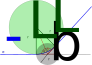
\includegraphics[height=0.3\columnwidth]{elecspec.png}\includegraphics[height=0.3\columnwidth]{Espec_shotexemp.jpg}
\includegraphics[width=0.75\columnwidth]{TrackingFigMangles2015.png}
\caption[Visualisation of an electron deflected in a homogeneous magnetic field and ]{Visualisation of an electron deflected in a homogeneous circular magnetic field (grey) with radius $r_b$. The larger green circle indicates the Larmor radius, determining the electron trajectory (blue) from the point of entry into the field (A) to its exit point (C) resulting in a total deflection $\theta$. Bottom: Example of particle tracking through a three-piece magnet for electrons of -X, 0 and +X MRAD pointing.}
\end{figure}
\SMComm{I suggest not filling the larmor orbit circle - there is nothing inside it, and it was easy to confuse with the b fiekdb}
\SMComm{Small numbers! Units!! }
Drawing the circular field region for the magnetic field and the electron entering the field, one can then graphically indicate its Larmor radius, equivalent to its expected motion for the region with the constant B-field. The angles in this geometry are determined using the trigonometric relation that the angles in a triangle have to add up to $\pi$:
\begin{equation}
2 \alpha + \theta = \pi,
\end{equation}
where $\theta$ is the deflection angle and $\alpha$ the angle indicated in the graphic (see figure).

Relating this to the angles to substitute $\alpha$:
\begin{equation}
\tan \alpha = \frac{r_L}{r_b},
\end{equation}
and then expressing this into parameters we can measure in experiment we reach
\begin{align}
\tan \frac{\theta}{2} &= \frac{r_b}{r_L},\nonumber\\
&= \frac{e B r_b}{p_\perp}.
\end{align}

In a typical LWFA experiment $p_\perp$ will be dominated by the component in the laser propagation axis, i.e. if the propagation axis were z, $|\mathbf{p_\perp}| \approx p_z$. 
\vspace{\baselineskip}

The correct assignment of the position on the screen to the correct electron energy is achieved by measuring the position of all components (lanex screen, magnet, TCC) and mapping the magnet field strength accurately, for instance using a Hall probe, and then running a particle tracking code with these details.
\SMComm{which one(s) were used in this thesis? }
Each pixel has a certain error bar on its associated energy as the divergence of the electron beam (instrument function), an offset at source or shot-to-shot pointing fluctuations could lead to different positions at the same electron energy (pointing). The energy resolution is determined by the strength of the magnetic field, the drift length, the intrinsic spatial resolution of the scintillator (for Lanex $\sim 100\,\mathrm{\mu m}$ REF) and the spatial resolution of the imaging system. 
\SMComm{A bit unclear, }
\vspace{\baselineskip}

A second Lanex screen or other spatial references (fiudicials) can help to identify and correct for pointing fluctuations or an overall pointing to achieve a more accurate determination of the energy, but could introduce additional scattering. 
\SMComm{What does overall pointing mean}
See \cite{PoderThesis} for more details on this or for instance \cite{Clayton2010_ION,Soloviev2011_TWOSCREEN}.

The width of the electron trace in the non-dispersion direction can be used to determine the divergence of the beam (in the non-dispersion axis) and cross-checked with the spectrum of the betatron radiation or a beam profile monitor.
\SMComm{How?}
\vspace{\baselineskip}

In addition to measuring the distances and the magnetic field, the imaging system for the scintillator screen has to be characterised.
This requires transforming the optical image (projective transform), spatially calibrate the image and translate from spatial to energy axis.
More details on the typical procedure can be found, for instance, in Jason Cole's or Kristjan Poder's PhD thesis \cite{ColeThesis, PoderThesis}
\SMComm{Why}
In all Chapters Lanex (standard and Biomax) are used in conjunction with Andor Neo cameras.

The signal recorded from the lanex screen can be related to the absolute number of electrons by cross calibrating with an imaging plate \cite{WoodThesis}.



\section{Gamma-ray Diagnostics}
\label{Methods:Sec:GammaDiags}

\subsection{Scintillator Profile Screen}

Once the energies reach the gamma-ray regime (> 1 MeV), even using an indirect-detection camera on axis becomes infeasible as photons will decay into secondary particles and radiation that will shower the camera and reduce its lifetime.

Relying on indirect detection with an off-axis camera or detector then becomes necessary. 
In experiment this has been an array of scintillator material normal to the beam axis and imaged by a camera.

This enables measuring the shape of the profile is interesting as it allows deduction of the source (SEE REF). In this context it gives insight into the properties of the electrons (their divergence, propagation and so on). 
The profile is also an indicator the the intensity of the interaction in non-linear ICS and carries the imprint of the interacting electron beam within it.
It is hence a useful diagnostic to not only confirm an interaction took place but also to characterise the conditions at the interaction.

\EliasComm{Reference REF UMSTADTER AO? TOM BLACKBURN IF PUBLISHED.}

\subsubsection{Experimental Implementation}

In these experiments caesium-iodide doped with thallium is used (TO DO WHAT REF NUM\addnum) frequently due to its high light yield. LANEX has typically a better spatial resolution due to its fine grain size ($\sim 100\,\mathrm{\mu m}$) but the energy deposition in the thin screens, especially at gamma-ray energies, is not sufficient to produce a lot of signal. Long CsI crystals give a pixelated response. LYSO also comes at a decent resolution but the light yield is lower. It is a fast scintillator but at lower repetition rates as at \textsc{Gemini}, this is not necessary and the noise levels can not be gated away as it is too close.
\SMComm{Sometimes the style is a bit to conversational.  “Comes at a decent resolution” is not very tight phrasing }
\begin{figure}
\centering
\includegraphics[height=0.3\columnwidth]{JenaProfile.jpg}\includegraphics[height=.3\columnwidth]{ScreenshotGEANT_JenaStack.png}\includegraphics[height=0.3\columnwidth]{20190208r015s036_GammaProfile_crop.jpg}
\caption[Scintillator profile screen, photograph, GEANT representation and measured gamma signal.]{Example of a scintillator stack used as profile screen in experiment. Photograph of the scintillator screen (left) along its GEANT representation (middle) and gamma signal measured with the stack in experiment (right).}
\end{figure}

Different profile screens were used in the experiments. The details can be found in Table XX NUMBER REF.

The scintillators emit around 546 nm (XX NUMBER) of radiation which is ideal for CCD chips. Andor iXon cameras (sensitive chips) are used to image the scintillators close to normal or using a mirror. A bandpass filter can be used to reduce the noise.


\begin{table}[h]
\centering
\begin{tabular}{l|l|l|l|r|r}
Name & Chapter &Crystals & Crystal Dimension & Front Plate & Divider\\ \hline \hline
QUB & \ref{Chap:BW}, BW & $20 \times 20$ & $2 \times 2 \times 20$ mm & Al 10 mm & Al 0.1 mm\\
Jena & \ref{Chap:linICS}, linICS & $45 \times 45$ & $1 \times 1 \times 10$ mm & TiO2 0.5 mm & TiO2 0.2 mm\\
DESY & \ref{Chap:linICS}, linICS & $30 \times 30$ & $1.5 \times 1.5 \times 10$ mm & Epoxy 0.5 mm & Epoxy 0.2 mm\\
RAL & \ref{Chap:RR15}, RR & $47 \times 33$ & $5 \times 5 \times 50$ mm & None & Al 1 mm
\end{tabular}
\caption[Overview of scintillator arrays used as profile screens in experiments.]{Overview of caesium-iodide crystal stacks used in experiments as profile screens.}
\end{table}

The photons go through the entire thickness of 10 mm CsI, so background subtraction from random noise was not a large concern. The signal is strong, also due to the high light yield of CsI at cost of spatial resolution (1mm crystals). The crystal outlines themselves and the overall array act as spatial reference as their symmetry is well known. A close to normal orientation is preferable to discourage mixing and again a normal imaging is ideal as well, resulting in very little post-processing being required.



\subsubsection{GEANT simulations showing energy deposition}
\SMComm{NIST is a good bridge as it goes up to the MeV level (Henke stops at 30 keV)}
\EliasComm{Add a figure on energy deposition using GEANT REF for MeV range and on the other hand absorption using Henke.}
RESULT: The energy deposited in an energy range (GIVE GEANT SIM FOR 10-XX MEV) is proportional to the energy of the radiation.

\EliasComm{Add comment on GEANT code in general, REF GEANT, mention Jason's and Kris' input.}

When planning to use such a detector as measurement of the total energy of the radiation one has to keep in mind that this is not a calorimeter in the gamma regime as radiation is bound to be transmitted through the stack. However, it is expected that the energy deposited per photon will vary and of course the number of photons will leave their trace on this detector.

The response is simulated using GEANT:
The detector in the simulation:
the detector assembled in the simulation is based on a CsI stack used in some experiments and provided by the Helmholtz Institut in Jena.
It consists of 45 x 45 CsI(Tl) crystals of face dimension 1 mm x 1 mm and a thickness of 10 mm. The crystals are spaced by a 0.2 mm layer of TiO2 and the front side has another layer of TiO2 of 0.5 mm which holds the entire stack together.

The stack was defined as such in the simulation and it can be seen in Figure ADD HERE.


The front side of the detector is XX m away from the source of the radiation, similarly to experiment conditions, hence being in general able to cover plus minus NUMBER divergence from a point source if centred along the same axis.

Now individual photons with ranging energy from 10 keV to 500 MeV are launched from the source point and the energy deposited in the crystals is being recorded. Each energy step is simulated 10000 to 100000 times and then averaged to obtain an average energy deposited per photon of this energy.

The results from these simulation can be seen in figure ADD HERE. Photon energies up to ENERGY are almost completely absorbed, backscattered and rarely transmitted. At around 200 keV suddenly a large amount of radiation is being absorbed. This indicates a material characteristic absorption edge.
This means that whilst for the majority of the energy ranges the CsI profile will give a good indication as energy times flux is monotonic increasing and somewhat linear for the two regimes of interest. In the regime of hundreds of keV we have to consider that a lot of energy will be absorbed in the front layer and we have to check how this behaves further downstream in the next detector.

\begin{figure}
\centering
\includegraphics[width=.5\columnwidth]{Edep_JenaStack.pdf}\includegraphics[width=.5\columnwidth]{Edep_JenaStack_rel.pdf}
\caption{Simulation results: energy deposited per photon in a profile stack. Replace this by 10's MeV plot as GEANT is not performing too well at low keV levels and the 250 keV peak might be a fluke.}
\end{figure}

If we look at this in terms of relative energy deposited per photon, so in other words energy deposited over energy of the photon, this does not look like a sharp edge but merely a steady decrease in energy deposited relative to the total photon energy. Scattering cross sections typically decrease with increase in energy and this goes along the same lines.


\subsubsection{Absolute Calibration}

The smaller profile stacks can also be calibrated by using a radioactive source since the stack mainly consists of crystals.
A Na or Cs source can be used at the standard measurement conditions. The energy emission is well known. If one assumes that all energy is absorbed by the detector the light yield is related to energy deposited. The disadvantage to real calorimeters is that due to a non-zero transmission through the material and due to the spacers not all energy deposited is deposited within crystals and converted into signal.
\SMComm{Which isotopes?}

